\documentclass[9pt, aspectratio=169]{beamer}
\usepackage{FiraSans}
\usetheme{metropolis}
\usepackage[utf8]{inputenc}
\usepackage{amsmath}
\usepackage{amsfonts}
\usepackage{amssymb}
\usepackage{multicol}
\usepackage{tikz}
\usepackage{xcolor}
\usepackage{subcaption}
\usepackage[T1]{fontenc} 
\usepackage[skins]{tcolorbox}
\author{Nicola Roman\`o - nicola.romano@ed.ac.uk}
\title{Image features}
\setlength{\fboxsep}{0pt}
\setbeamertemplate{caption}{\raggedright\insertcaption\par}
\setbeamertemplate {footline}{\begin{scriptsize}\hfill\insertframenumber ~of \inserttotalframenumber\kern1em\vskip5pt\end{scriptsize}}

%\setbeamercovered{transparent} 
%\setbeamertemplate{navigation symbols}{} 

\titlegraphic{\centering \includegraphics[scale=.5]{instituteLogo.png}}
\date{}

\AtBeginSection[]
{
  \begin{frame}<beamer>
    {Outline}
    \huge{\tableofcontents[currentsection]}
  \end{frame}
}

\AtBeginSubsection[]
{
  \begin{frame}<beamer>
    {Outline}
    \huge{\tableofcontents[currentsection, currentsubsection]}
  \end{frame}
}

\begin{document}

\newtcolorbox{codebox}{enhanced,
    top=2pt,
    left=2pt,
    right=2pt,
    bottom=2pt,
    boxrule=0pt,
    leftrule=5pt,
    sharp corners,
    colback=gray!20,
    colframe=blue!60!black}

\begin{frame}
    \titlepage
\end{frame}

\begin{frame}
    {Learning objectives}
    \begin{columns}
        \begin{column}{0.8\textwidth}
            \begin{itemize}
                \item Define and give examples of image features
                \item Describe and apply methods for detection of shapes in an image
                \item Describe and apply methods for particle detection
                \item Discuss advantages and issues with these methods
            \end{itemize}
        \end{column}
        \begin{column}{0.2\textwidth}
            
\includegraphics[angle=-30, origin=tr, width=1.5\textwidth]{lightbulb.png}
        \end{column}
    \end{columns}
\end{frame}

\section{What is a feature?}

\begin{frame}
    {Features}
    \textbf{Feature}, n.: a distinctive or characteristic part of a thing; some part which arrests the attention by its conspicuousness or prominence.\\
    (\textit{Source: Oxford English Dictionary})
    \pause

    \vspace{2em}

    In image analysis, a \textbf{feature} is a characteristic of the image, or of a part of it, that defines some of its properties.

    Examples of features include edges, corners, ridges, texture, colour, shape etc.

    \pause
    \vspace{2em}
    Detecting features is a fundamental step to extract information from images.
\end{frame}

\begin{frame}
    {Features in images}
    \begin{figure}
        \includegraphics[width=\textwidth]{mountain.jpg}
        \caption{\small{\color{gray}{View in the Gran Sasso mountain range, Italy - Photo: Nicola Roman\`o}\color{black}}}
    \end{figure}
    \centering
    \textbf{Which are the prominent features of this image?}
\end{frame}

\section{Geometric features}

\begin{frame}
    {Geometric features}
    \centering
    Examples of \textbf{geometric features} include:\\
    \vspace{2em}

    \begin{figure}
        \centering
        \subcaptionbox{\centering \textbf{Blobs} - \color{gray}{Marsh et al., Sci Rep 2018}}
        {\includegraphics[width=.22\textwidth]{AFM - Marsh 2018.png}}
        \subcaptionbox{\centering \textbf{Corner and edges} (see lecture 5) - \color{gray}{Credits: Masur, Wikipedia, CC-0}}
        {\includegraphics[width=.22\textwidth]{yeast.png}}
        \subcaptionbox{\centering \textbf{Lines, circles, etc.} - \color{gray}{Credits: Vivien Rolfe, Flickr, CC-BY-SA-2.0}}
        {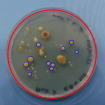
\includegraphics[width=.22\textwidth]{plate.png}
        }
        \subcaptionbox{\centering \textbf{Ridges} - \color{gray}{Credits:  Medical gallery of Mikael H\"aggstr\"om., CC-0}}
        {\includegraphics[width=.22\textwidth]{retina_vessels.png}}
    \end{figure}
\end{frame}

\subsection{Blobs}

\begin{frame}
    {Blob detection}
    Blob detection is the task of detecting blobs in an image.

    \textbf{Blobs} are defined as regions of pixels with uniform properties that are clearly distinguishable from the background.

    There are many methods for detecting blobs in an image; today we will look at using the Laplacian of the Gaussian (\textbf{LoG}) method, and its approximation by the difference of Gaussians (\textbf{DoG}) method.
\end{frame}

\begin{frame}
    {The Laplacian operator}
    In the last lecture we used the first-order derivatives of the image (the gradient) to detect edges. This time we will look at the second order derivatives.

    \pause
    We define the \textbf{laplacian} of an image as the sum of the second order partial derivatives of the image.
    \large{
    $$\text{Laplacian(I)} = \nabla^2(I) = \frac{\partial^2{I}}{\partial{x^2}} + \frac{\partial^2{I}}{\partial{y^2}}$$
    }
\end{frame}

\begin{frame}
    {The Laplacian of the Gaussian}
    What does the Laplacian of a Gaussian function look like?

    \begin{figure}
        \centering
        \includegraphics[width=.45\textwidth]{gaussian_and_laplacian_2D.png}
        \includegraphics[width=.45\textwidth]{gaussian_and_laplacian_3D.png}
    \end{figure}

    So... how do we use this to detect blobs?
\end{frame}

\begin{frame}
    {The LoG method for blob detection}
    The idea is to:

    \begin{enumerate}
        \item Apply a Gaussian filter  $G(\sigma)$ to the image
        \item Calculate the Laplacian of the Gaussian-filtered image
              \pause
        \item Dark blobs on light background will appear as bright spots in the Laplacian of the Gaussian-filtered image; bright blobs on dark background will appear as dark spots.
              \pause
        \item We find local maxima (or minima) in the Laplacian of the Gaussian-filtered image to determine the position of the blobs
        \item The blob size is approximately $\sqrt{2}\sigma$
    \end{enumerate}
\end{frame}

\begin{frame}
    {The DoG method for blob detection}
    To detect blobs of different size, we can use a Gaussian filter with different standard deviations.

    \pause
    \only<2>{\includegraphics[width=\textwidth]{blob_detection_thr0.png}}
    \only<3>{\includegraphics[width=\textwidth]{blob_detection_thr0_4.png}}
    \only<4->{\includegraphics[width=\textwidth]{blob_detection_thr0_8.png}}

    \only<2->{We can apply a threshold to the DoG image to remove spurious blobs and can also remove blobs overlapping over a certain \%.}

    \only<5>{Scikit image implements these steps in the \href{https://scikit-image.org/docs/dev/api/skimage.feature.html\#skimage.feature.blob\_log}{\texttt{skimage.feature.blob\_log}} function}.
\end{frame}

\begin{frame}
    {Example of blob detection}
    \begin{columns}
        \begin{column}{.7\textwidth}
            \begin{codebox}
                \texttt{from skimage.feature import blob\_log\\
                    from skimage.io import imread\\
                    \\
                    nucleus = imread("nucleus\_blob.png")\\
                    blobs = blob\_log(nucleus, min\_sigma=10, max\_sigma=15,
                    $~~~~~~~~~~~~~~~~~$num\_sigma=5, threshold=0.3, overlap=.4)\\
                    \pause
                    plt.imshow(nucleus, cmap="gray")\\
                    \\
                    for b in blobs:\\
                    $~~~~$y, x, radius = b\\
                    $~~~~$\# Create a circle at the blob center\\
                    $~~~~$c = plt.Circle((x, y), radius, color='orange',
                    $~~~~~~~~~~~~~~~~~~~$linewidth=3, fill=False)\\
                    $~~~~$\# Draw the circle (gca = "get current axis")\\
                    $~~~~$plt.gca().add\_artist(c)\\
                    plt.show()
                }
            \end{codebox}
        \end{column}
        \begin{column}{.3\textwidth}
            \only<2>{
                \includegraphics[width=\textwidth]{blob_log_example.png}
            }
        \end{column}
    \end{columns}
\end{frame}

\begin{frame}
{Other methods for blob detection}
Scikit image impements two other methods for blob detection: the DoG (Difference of Gaussians) and the DoH (Determinant of the Hessian) methods.

\pause

The \textbf{DoG method} is a fast approximation of the LoG method. It works by calculating the difference between two version of the image blurred by Gaussians with different $\sigma$.

The \textbf{DoH method} is the fastest method. It works by calculating the determinant of the Hessian of the image (the \href{https://en.wikipedia.org/wiki/Hessian\_matrix}{\underline{Hessian}} is a matrix of second partial derivatives).
Contrary to DoG and LoG, the detection speed is independent of the size of the blobs. However, DoH is less accurate at detecting small blobs.

\pause
These are implemented in \href{https://scikit-image.org/docs/dev/api/skimage.feature.html\#skimage.feature.blob\_dog}{\texttt{\underline{skimage.feature.blob\_dog}}} and \href{https://scikit-image.org/docs/dev/api/skimage.feature.html\#skimage.feature.blob\_doh}{\texttt{\underline{skimage.feature.blob\_doh}}} respectively.
\end{frame}

\subsection{Lines and circles (the Hough transform)}

\begin{frame}
    {The Hough transform}
    The Hough transform is a technique originally developed by Paul Hough in 1962 for finding straight lines in an image. Extensions of this technique allow to find circles and quadrilaterals.
    \centering
    \includegraphics[width=.85\textwidth]{hough_line_overview.png}
\end{frame}

\begin{frame}
    {Representing a line}
    \begin{columns}
        \begin{column}{.5\textwidth}
            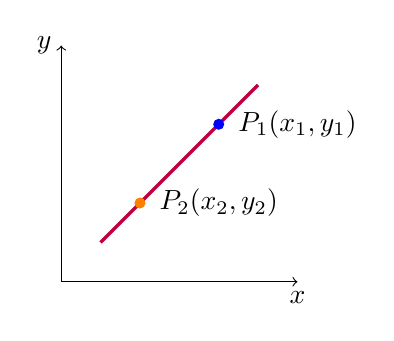
\begin{tikzpicture}
                \draw[thin,->] (0,0) -- (3,0) node[below] {$x$};
                \draw[thin,->] (0,0) -- (0,3) node[left] {$y$};
                \draw[purple, very thick] (0.5, 0.5) -- (2.5, 2.5);
                \fill [orange] (1, 1) circle (2pt);
                \fill [blue] (2, 2) circle (2pt);
                \node at (3, 2) {$P_1(x_1, y_1$)};
                \node at (2, 1) {$P_2(x_2, y_2$)};
            \end{tikzpicture}

            Consider a line with equation: $y = a\cdot x + b$ and two points $P_1$ and $P_2$ on it.
        \end{column}
        \pause
        \begin{column}{.5\textwidth}
            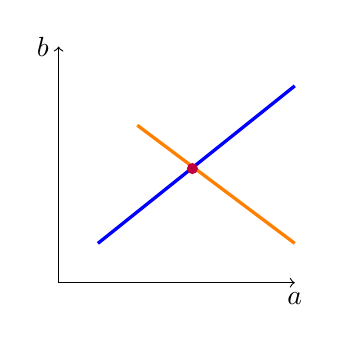
\begin{tikzpicture}
                \draw[thin,->] (0,0) -- (3,0) node[below] {$a$};
                \draw[thin,->] (0,0) -- (0,3) node[left] {$b$};
                \draw [orange, very thick] (1, 2) -- (3, 0.5);
                \draw [blue, very thick] (0.5, 0.5) -- (3, 2.5);
                \fill [purple] (1.7, 1.45) circle (2pt);
                % \fill [blue] (2, 1) circle (2pt);
                % \node at (2, 2) {($x_1, y_1$)};
                % \node at (3, 1) {($x_2, y_2$)};
            \end{tikzpicture}

            The families of lines passing through $P_1$ (or $P_2$) have equation: $b = - x_1\cdot a + y_1$ (or $b = - x_2\cdot a + y_2$).
            \pause
        \end{column}
    \end{columns}

    The intersection is the slope and intercept of the original line! Any point on the red line on the left will correspond to a line passing through the red point in the $a/b$ space.\\
    \textbf{This is the principle of the Hough transform.}
\end{frame}

\begin{frame}
    {Representing a line - another way}
    We can also represent a line in terms of an angle and a distance from the origin. This is a better alternative, because we can also use it to represent a vertical line.\\

    \large
    \begin{center}
        $x \cdot \cos(\theta) + y \cdot \sin(\theta) = \rho$
    \end{center}

    \begin{columns}
        \begin{column}{.5\textwidth}
            \normalsize
            Where $\theta$ is the angle of the line and $rho$ is the distance from the origin.

            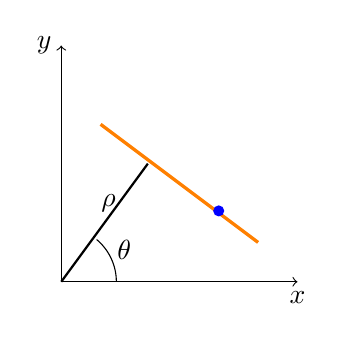
\begin{tikzpicture}
                \draw[thin,->] (0,0) -- (3,0) node[below] {$x$};
                \draw[thin,->] (0,0) -- (0,3) node[left] {$y$};
                \draw [thick] (0, 0) -- (1.1, 1.5);
                \draw [orange, very thick] (0.5, 2) -- (2.5, 0.5);
                \draw (0.7, 0) arc (0:50:.7) node at (.8, .4) {$\theta$}
                ;
                \node at (.6, 1) {$\rho$};
                \fill [blue] (2, 0.9) circle (2pt);
            \end{tikzpicture}
        \end{column}
        \pause
        \begin{column}{.5\textwidth}
            \normalsize
            We can map each point in the $\theta/\rho$ space (called the Hough space) as we did before.

            \begin{tikzpicture}
                \draw[thin,->] (0,0) -- (3,0) node[right] {$\theta$};
                \draw[thin,->] (1.4,0) -- (1.4,3) node[left] {$\rho$};
                \node at (0, -.2) {$-\pi$};
                \node at (2.8, -.2) {$\pi$};
                \draw [blue] plot [smooth, tension=1.2] coordinates { (0,2.4) (0.5, 2.2) (1,1.6) (2,0.5) (2.9,0.7)};
            \end{tikzpicture}
        \end{column}
    \end{columns}
\end{frame}

\begin{frame}
    {The Hough transform}
    There are three steps in the Hough transform:

    \begin{enumerate}[<+->]
        \item Edge detection - e.g. using the Canny edge detector. This gives us a binary image.
        \item We create a $M x N$ matrix of 0s, representing the Hough space. This will correspond to $M$ different values of $\rho$ and $N$ different values of $\theta$.
        \item Iterate through all the pixels of the image and if they are an edge map they get to "cast a vote" onto the Hough space.
        \item Each value in the Hough space matrix is use as an "accumulator". We add 1 to the value of the Hough space at the corresponding $\theta$ and $\rho$ coordinates for each possible line passing through the edge point.
        \item The Hough space matrix is then thresholded and non-maximum-suppression applied to find the strongest lines.
    \end{enumerate}
\end{frame}

\begin{frame}
    {Hough transform - an example}
    \only<1>{
        \begin{codebox}
            \texttt{from skimage.feature import canny\\
                from skimage.transform import hough\_line, hough\_line\_peaks\\
                \\
                chamber = imread("cell\_counting\_chamber.jpg")\\
                chamber\_canny = canny(chamber, sigma=1.5)}
        \end{codebox}
        \centering
        \includegraphics[width=.6\textwidth]{chamber_and_canny.png}
    }
    \only<2>{
        \begin{codebox}
            \texttt{hough\_space, angles, d = hough\_line(chamber\_canny)\\
            accum, theta, rho = hough\_line\_peaks(hough\_space, angles, d)\\
            for t, r in zip(theta, rho):\\
            $~~~~$print(f"{np.rad2deg(t):0.2f}, {r:0.2f}")
            }
        \end{codebox}
        \begin{columns}
            \begin{column}{.7\textwidth}
                \centering
                \includegraphics[width=.7\textwidth]{chamber_hough_space.png}
            \end{column}
            \begin{column}{.23\textwidth}
                \begin{codebox}
                    \texttt{88.99, 253.77\\
                        88.99, 97.60\\
                        -1.51, 258.77\\
                        -1.51, 171.68\\
                        88.99, 332.85\\
                        -1.51, 84.59\\
                        88.99, 172.68\\
                        -1.51, 0.50\\
                        88.99, 23.52
                    }
                \end{codebox}
            \end{column}
        \end{columns}

    }
\end{frame}

\section{Texture features}

\begin{frame}
    {Basic texture features}
    Range, variance
\end{frame}

\begin{frame}
    {GLCM}
\end{frame}

\begin{frame}
    {HOG features}
\end{frame}
\end{document}

